\documentclass[11pt, handout]{beamer}
\usetheme{Berlin}
\usecolortheme{dolphin}
\usepackage[utf8]{inputenc}
\usepackage[francais]{babel}
\usepackage{amsmath}
\usepackage{amsfonts}
\usepackage{amssymb}
\usepackage{hyperref}

\setbeamertemplate{caption}{\raggedright\insertcaption\par\scriptsize}
\author{Nicolas Kobel \\Raphael Racine}
\title{Vaccin Peptidique contre \textit{H. Pylori}}
\subtitle{Presentation intermediaire}
%\setbeamercovered{transparent} 
%\setbeamertemplate{navigation symbols}{} 
%\logo{img/logo.png} 
%\institute{} 
%\date{} 
%\subject{} 

%\usebackgroundtemplate%
%{%
%    \includegraphics[height=\paperheight]{img/logo.png}%
%}

\newcommand{\hpyl}{\textit{H. Pylori}}
\begin{document}

\begin{frame}
\titlepage
\end{frame}

\begin{frame}
\tableofcontents
\end{frame}

\section{H. Pylori}
\begin{frame}
\frametitle{\hpyl}
\begin{columns}[c]
	\begin{column}[c]{5cm}
		\begin{itemize}[<+->]
			\item Helicobacter pylori
			\item Muqueuses Estomac
			\item Urease
			\item Modification environnement
			\item Ulcers, Cancers
		\end{itemize}
	\end{column}
	\begin{column}[c]{5cm}
	\begin{figure}
		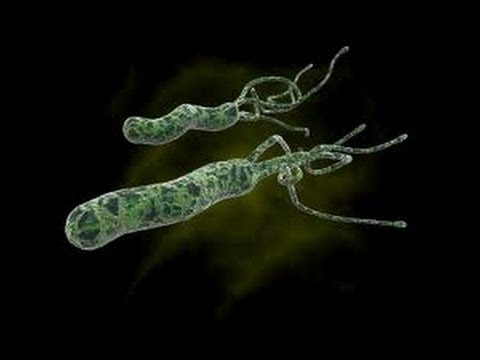
\includegraphics[width=\textwidth]{img/hpylori.jpg}
		\caption{\href{https://i.ytimg.com/vi/DYzYLTRASRM/hqdefault.jpg}{source}}
	\end{figure}
	
	\end{column}
\end{columns}
%\note{
%Description de la bacterie et de ses méchanismes de défenses et d'attaque
%}
\end{frame}

\section{Urease}
\begin{frame}
\frametitle{Urease}
\framesubtitle{Description Générale}
\begin{columns}[c]
	\begin{column}[c]{5cm}
		\begin{itemize}[<+->]
			\item Enzyme
			\item Transforme l'urée
			\item Utilisée pour l'identification bactérienne
		\end{itemize}
	\end{column}
	\begin{column}[c]{5cm}
		\begin{figure}
		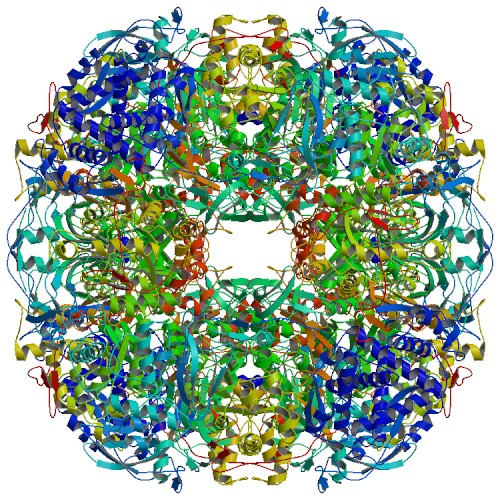
\includegraphics[width=\textwidth]{img/urease.jpg}
		\caption{\href{http://www.rcsb.org/pdb/images/1E9Z_bio_r_500.jpg}{source}}
	\end{figure}
	\end{column}
\end{columns}
\end{frame}

\begin{frame}
\frametitle{Urease}
\framesubtitle{Urease $\alpha$ et $\beta$}
\begin{columns}[c]
	\begin{column}[c]{5cm}
		\begin{itemize}[<+->]
			\item Sous-unités de l'urease
			\item $\alpha$ : Site actif
			\item $\beta$ : Site d'identification
			\item $\beta$ : 5 Mutations
		\end{itemize}
	\end{column}
	\begin{column}[c]{5cm}
	\begin{figure}
		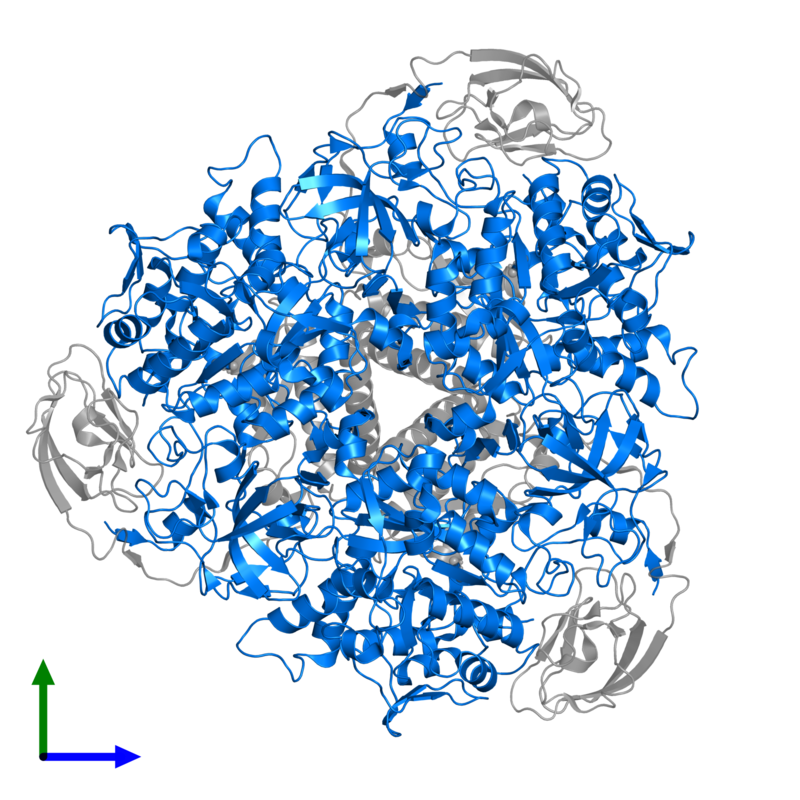
\includegraphics[width=\textwidth]{img/ureasealpha}
		\caption{\href{http://www.ebi.ac.uk/pdbe/static/entry/1a5n_entity_3_front_image-800x800.png}{source}}
	\end{figure}
	\end{column}
\end{columns}
\end{frame}

\section{Vaccins Péptidiques}
\begin{frame}
\frametitle{Vaccins Péptidiques}
\framesubtitle{Vaccins}
\begin{columns}[c]
	\begin{column}[c]{5cm}
		\begin{itemize}[<+->]
			\item Entrainement système immunitaire
			\item Identification de parasites
			\item Microbes affaiblis ou morts
		\end{itemize}
	\end{column}
	\begin{column}[c]{5cm}
		\begin{figure}
		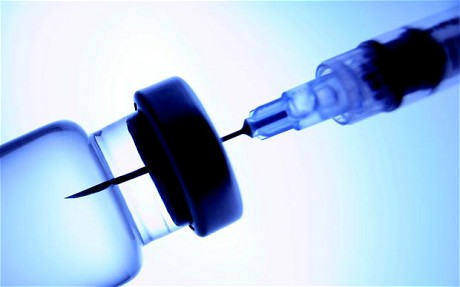
\includegraphics[width=\textwidth]{img/vaccine}
		\caption{\href{http://vaccineresistancemovement.org/wp-content/uploads/2010/05/Universal-Flu-Vaccine1.jpg}{source}}
	\end{figure}
	\end{column}
\end{columns}
\end{frame}

\begin{frame}
\frametitle{Vaccins Péptidiques}
\framesubtitle{Vaccins Péptidiques}
\begin{columns}[c]
	\begin{column}[c]{5cm}
		\begin{itemize}[<+->]
			\item Peptides
			\item Identificateurs de la Bactérie
			\item Synthetisable
			\item Pas besoin de bactérie affaiblie
		\end{itemize}
	\end{column}
	\begin{column}[c]{5cm}	
		\begin{figure}
		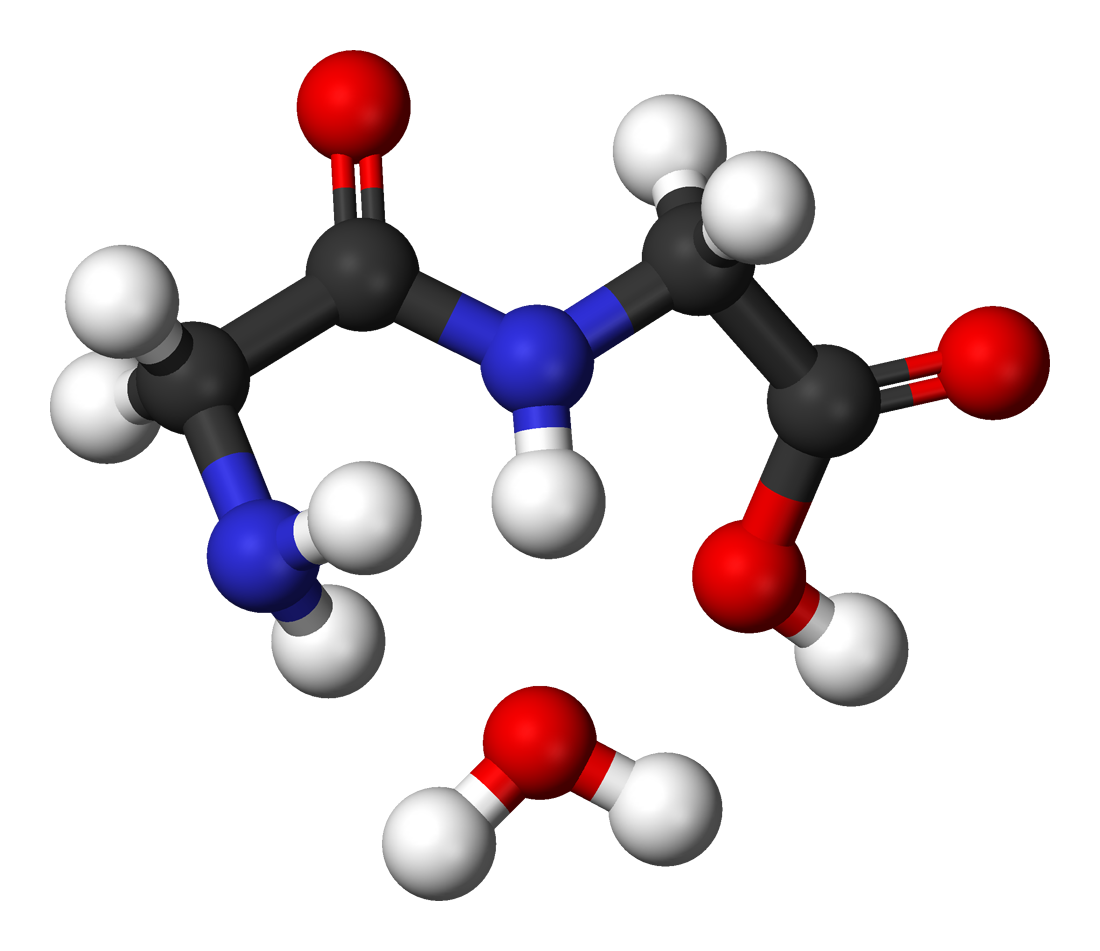
\includegraphics[width=\textwidth]{img/peptide}
		\caption{\href{https://upload.wikimedia.org/wikipedia/commons/9/94/Glycine-condensation-2-3D-balls.png}{source}}
	\end{figure}
	\end{column}
\end{columns}
\end{frame}

\section{Etat de l'art}
\begin{frame}
\frametitle{Etat de l'art}
\framesubtitle{Diagnostique}
\begin{columns}[c]
	\begin{column}[c]{5cm}
		\begin{itemize}[<+->]
			\item Peines Abdominales
			\item Nausées et Vaumissements
			\item Anémie
		\end{itemize}
	\end{column}
	\begin{column}[c]{5cm}
		\begin{itemize}[<+->]
			\item Tests de l'haleine
			\item Tests sanguins
			\item Examen des selles
			\item Biopsies
		\end{itemize}
	\end{column}
\end{columns}
\end{frame}

\begin{frame}
\frametitle{Etat de l'art}
\framesubtitle{Traitement}
\begin{columns}[c]
	\begin{column}[c]{5cm}
		\begin{itemize}[<+->]
			\item Antibiotique
			\item Inhibiteur de Pompe à Protons
			\item Traitement triple
		\end{itemize}
	\end{column}
	\begin{column}[c]{5cm}
	\begin{figure}
		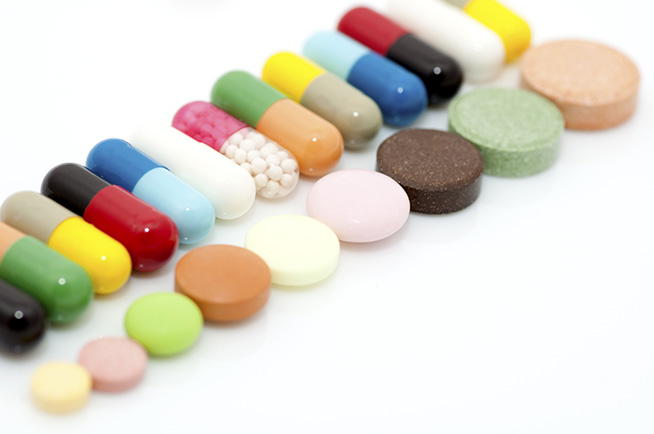
\includegraphics[width=\textwidth]{img/antibiotics}
		\caption{\href{http://www.rebootwithjoe.com/wp-content/uploads/2014/02/Antibiotics.jpg}{source}}
	\end{figure}
	\end{column}
\end{columns}
\end{frame}

\begin{frame}
\frametitle{Etat de l'art}
\framesubtitle{Prévention}
\begin{columns}[c]
	\begin{column}[c]{5cm}
		\begin{itemize}[<+->]
			\item Empêcher Prolifération
			\item Vaccins testés en Chine
			\item Vaccin polypétpique Munich
		\end{itemize}
	\end{column}
	\begin{column}[c]{5cm}
		\begin{figure}
		
\includegraphics[width=\textwidth]{img/who}
		\caption{\href{http://www.unngls.org/images/areas-of-work/WHO.jpg}{source}}
	\end{figure}
	\end{column}
\end{columns}
\end{frame}

\begin{frame}
\frametitle{Etat de l'art}
\framesubtitle{Prédiction d'épitopes}
\begin{columns}[c]
	\begin{column}[c]{5cm}
		\begin{itemize}[<+->]
			\item Sequence Based Prediction
			\item Structure Based Prediction
			\item Hybrid Methods
			\item Consensus from multiple Methods
		\end{itemize}
	\end{column}
	\begin{column}[c]{5cm}
	\end{column}
\end{columns}
\end{frame}

\begin{frame}
\frametitle{Etat de l'art}
\framesubtitle{Prédiction d'épitopes linéaire}
\begin{columns}[c]
	\begin{column}[c]{5cm}
		\begin{itemize}[<+->]
			\item séquence $\rightarrow$ structure
			\item structure identique $\rightarrow$ fonction identique
		\end{itemize}
	\end{column}
	\begin{column}[c]{5cm}
		\begin{itemize}[<+->]
			\item Matrices Quantitatives (QM)
			\item Support Vector Machines (SVM)
			\item Artificial neural network (ANN)
			\item HMM, evolutionary algorithms, \ldots
		\end{itemize}
	\end{column}
\end{columns}
\end{frame}

\section{Réalisation}
\begin{frame}
\frametitle{Travail futur}
\begin{columns}[c]
	\begin{column}[c]{5cm}
		\begin{itemize}[<+->]
			\item Prédiction d'épitopes
			\item Vérification des épitopes
			\item Liste des péptides candidats
		\end{itemize}
	\end{column}
	\begin{column}[c]{5cm}
		
	\end{column}
\end{columns}
\end{frame}


\section{Questions}
\begin{frame}
\frametitle{Questions}
		\begin{figure}
		
\includegraphics[height=0.8\textheight]{img/questions}
		%\caption{\href{http://www.unngls.org/images/areas-of-work/WHO.jpg}{source}}
	\end{figure}
\end{frame}

\end{document}

\section*{sources}
\begin{frame}
\frametitle{sources}
\end{frame}